\section{Abstract Interpretation}
\label{bg:sec:abstract_interpretation}

As our way of living is becoming increasingly dependent on programs, errors
in safety-critical system can incur huge expenses, and even costs of lives.
For example, the maiden flight of Ariane 5 resulted in a failure, because of
a software instruction failed to convert a 64-bit floating-point number into
16-bit signed integer, as the result is too large to be represented by a 16-bit
signed integer~\cite{dowson97}.  The Patriot defense system failed to intercept
an incoming missile because of an accumulated round-off error in the system's
internal clock, resulted in the deaths of 28 people in 1991~\cite{patriot}.
\emph{Static analysis}, a process of analyzing a piece of program written in
an HLL without executing it, is therefore a research topic of great importance
to prevent similar catastrophic errors and mitigate costs of failure in the
future.

It is unfortunate that because of the halting problem~\cite{turing37} and
a direct consequence of it, Rice's theorem~\cite{rice53}, any nontrivial
property on the outcome of a program is in general undecidable.  It means
that an interesting property---a yes or no question---which is never
always true or always false for all programs, is \emph{undecidable}, or
in other words, cannot be answered.  Even a question as simple as ``does
this program return zero'' is difficult to answer.  A static analyzer can
therefore produce an answer which is either a definite ``yes'' or ``I don't
know''~\cite{mine04}, and designing one which answers a ``yes''.  Producing a
meaningful ``yes'' in an efficient manner poses a challenging task to static
analyzers.  Static analyzers rely heavily on formal techniques to perform
well.  Typical techniques employed include symbolic execution, model checking,
satisfiability modulo theories~\cite{demoura08}, data-flow analysis based on
lattices~\cite{nielson99}, and abstract interpretation~\cite{cousot77}.

This section starts by introducing the data-flow analysis framework to analyze
a simple program, abstract interpretation is then applied to this example, and
the properties of the resulting analysis are further discussed.

% This is then extended to define a scalable analysis capturing accuracy.
% Later in Chapter~\ref{chp:progopt} we accommodate sequential statements,
% \iflit~branches and \whilelit~loops in the accuracy analysis, and in
% Chapter~\ref{chp:latopt}, we further improve our analysis by supporting
% multi-dimensional arrays.

\subsection{Data-Flow Analysis Framework}
\label{bg:sub:data_flow}

\begin{figure}[ht]
    \centering
    \begin{minipage}{0.5\textwidth}
    \begin{lstlisting}
    float simple(float x)
    {
        while (x > 1.0)
            x *= 0.9;
        return x;
    }
    \end{lstlisting}
    \end{minipage}
    \caption{%
        A simple program example to be statically analyzed.
    }\label{bg:lst:simple}
\end{figure}
In this section, we use the \emph{data-flow analysis} (DFA)
framework~\cite{nielson99} to statically analyze a program named \verb|simple|
in Figure~\ref{bg:lst:simple}, which consists of only one variable \verb|x|.
We further assume an initial set $\iota \subseteq \realset$ of values of
\verb|x|, and the property that concerns us is answering whether a particular
value $x_\mathrm{invalid}$ is not in the set of all reachable final values
of \verb|x|.  A sensible definition for the set of values can be reached
by \verb|x| is a subset of all real numbers $\realset$, \ie~an element of
$\powersetof\realset$, where $\powersetof\realset$ denotes the \emph{power set}
of $\realset$, also known as the set of all subsets of $\realset$.

The first step of DFA is to translate the body of \verb|simple| into a
control/data-flow graph (CDFG), as shown in Figure~\ref{bg:fig:cdfg} where
each block consists of a single statement or conditional, and the edges in
the graph model the data- and control-flows.  The \textbf{tt} and \textbf{ff}
respectively highlight the control-flow branch taken when the conditional
\mbox{``\texttt{x < 1}''} evaluates to either true or false.
\begin{figure}[ht]
    \centering
    \tikzstyle{block} = [
        draw,
        fill=white,
        rectangle,
        minimum height=2em,
        minimum width=4em
    ]
    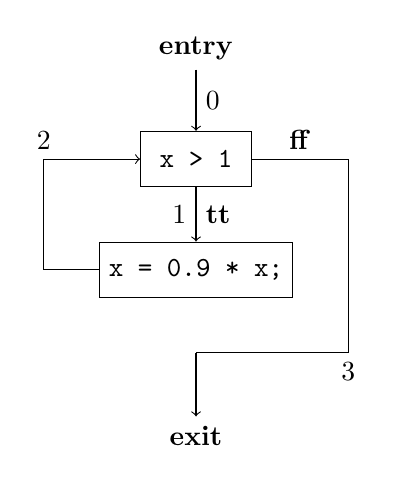
\begin{tikzpicture}[node distance=4em]
        \node(entr) {\textbf{entry}};
        \node(cond) [block, below of=entr] {\texttt{x > 1}};
        \node(stmt) [block, below of=cond] {\texttt{x = 0.9 * x;}};
        \node(midl) [coordinate, left of=stmt, xshift=-1.5em] {};
        \node(midr) [coordinate, right of=stmt, xshift=1.5em] {};
        \node(rtrn) [coordinate, below of=stmt, yshift=1em]
            {\texttt{return x;}};
        \node(exit) [below of=rtrn, yshift=1em] {\textbf{exit}};
        \draw[->] (entr) -- node[auto]{0} (cond);
        \draw[->] (cond) -- node[right]{\textbf{tt}} node[left]{1} (stmt);
        \draw[- ] (stmt) -- (midl);
        \draw[->] (midl) |- node[auto]{2} (cond);
        % \draw[->] (stmt) to[out=180, in=180] (cond);
        \draw[- ] (cond) -| node[auto, near start]{\textbf{ff}} (midr);
        \draw[- ] (midr) |- node[auto]{3} (rtrn);
        % \draw[->] (cond) to[out=0, in=0] (rtrn);
        \draw[->] (rtrn) -- (exit);
    \end{tikzpicture}
    \caption{%
        The CDFG of \texttt{simple} in Figure~\ref{bg:lst:simple}.
    }\label{bg:fig:cdfg}
\end{figure}

The individual blocks in the CDFG can therefore be defined as functions $f:
\powersetof\realset \to \powersetof\realset$ that admits an $S$ and produces
$T$, where both $S$ and $T$ are elements of $\powersetof\realset$.  For
instance, for the statement ``\texttt{x *= 0.9;}'', a function $f_1$ can be
defined as follows:
\begin{equation}
    f_1(S) = \{ 0.9 v \mid v \in S \}.
\end{equation}
Here, the definition of $f_1$ indicates that for all possible input values
$v$ of \verb|x| in the set $S$, we multiply it by $0.9$ and collect the
multiplied results into a new set as the output of $f_1$.  Similarly, because
\mbox{``\texttt{x > 1}''} has two conditional branches, two functions,
$f_{2,\truelit}$ and $f_{2, \falselit}$, respectively for both true- and
false-branches of it can be defined:
\begin{equation}
    \begin{aligned}
        f_{2, \truelit}(S) &= S \cap \{ v \in \realset \mid v > 1 \}, \\
        f_{2, \falselit}(S) &= S \cap \{ v \in \realset \mid v \leq 1 \}.
    \end{aligned}
\end{equation}
where $X \cap Y$ computes the intersection of the two sets $X$ and $Y$.

In the next step, the edges of the CDFG are labelled with numbers 0, 1, 2
and 3 to signify different locations of the program.  For each edge labelled
$i$, it is now possible to compute an $A(i)$, a set of values that could be
reached by \verb|x| in a program execution at each location $i$, by wiring up
the functions $f_1$, $f_{2, \truelit}$ and $f_{2, \falselit}$ that correspond
to program statements.  This gives rise to the following system of data-flow
equations:
\begin{align}
    A(0) &= \iota,
        \label{bg:eq:dfa0} \\
    A(1) &= f_{2, \truelit}(A(0) \cup A(2)),
        \label{bg:eq:dfa1} \\
    A(2) &= f_1(A(1)),
        \label{bg:eq:dfa2} \\
    A(3) &= f_{2, \falselit}(A(0) \cup A(2)),
        \label{bg:eq:dfa3}
\end{align}
where $A(0) \cup A(1)$ is the union of $A(0)$ and $A(1)$.

Unfortunately, computationally solving this system of equations is not an
easy task.  In Sections~\ref{bg:sub:most_precise} and~\ref{bg:sub:intervals},
the two significant impediments are explained, and subsequently, theories are
introduced to unravel them.


\subsection{The Most Precise Solution to a Data-Flow Equation}
\label{bg:sub:most_precise}

There are multiple solutions to this system.  For example, we can solve
it manually by substituting $A(0)$ and $A(2)$ in~\eqref{bg:eq:dfa1}
with~\eqref{bg:eq:dfa0} and~\eqref{bg:eq:dfa2}.  We arrive at:
\begin{equation}
    A(1) = \left(
        \iota \cup \left\{ 0.9 v \mid v \in A(1) \right\}
    \right) \cap \{ v \in \realset \mid v > 1 \}.
    \label{bg:eq:dfa_a1}
\end{equation}
It turns out that the set of all real numbers greater than $1$, or:
\begin{equation}
    A(1) = \{ v \in \realset \mid v > 1 \}
    \label{bg:eq:a11}
\end{equation}
is a solution to~\eqref{bg:eq:dfa_a1}.  Substituting $A(1)$ in the right-hand
side of~\eqref{bg:eq:dfa_a1} with this value proves that it is indeed the
solution for this equation, assuming all sets below are subsets of $\realset$
to simplify the derivation:
\begin{equation}
    \begin{aligned}
        A(1)
        &= \bigg( \iota \cup \Big\{ 0.9 v \mid v \in
                \left\{ v^\prime \mid v^\prime > 1 \right\}
           \Big\} \bigg) \cap \{ v \mid v > 1 \} \\
        &= \bigg( \iota \cup \left\{ 0.9 v \mid v > 1 \right\} \bigg) \cap
           \{ v \mid v > 1 \} \\
        &= \bigg( \iota \cup \left\{ v \mid v > 0.9 \right\} \bigg) \cap
           \{ v \mid v > 1 \} \\
        &= \bigg( \iota \cap \{ v \mid v > 1 \} \bigg) \cup
           \bigg(
               \left\{ v \mid v > 0.9 \right\} \cap \{ v  \mid v > 1 \}
           \bigg) \\
        &= \bigg( \iota \cap \{ v \mid v > 1 \} \bigg) \cup
           \{ v \mid v > 1 \} \\
        &= \{ v \mid v > 1 \}.
    \end{aligned}
\end{equation}

Intuitively, a manual inspection of \verb|simple| finds that \verb|x| can reach
values $v$, $0.9 v$, $0.9^2 v$, and \textellipsis, such that all values in this
sequence are greater than $1$, for each $v \in \iota$; or more succinctly, an
alternative solution to $A(1)$ should be:
\begin{equation}
    A(1) = \{ v \in \iota \mid 0.9^k v > 1 \wedge k \in \naturalset \}.
    \label{bg:eq:a12}
\end{equation}
Here $k \in \naturalset$ denotes $k$ is one of $0, 1, 2, \mathellipsis$, \ie~a
natural number.

It is evident to us the latter solution~\eqref{bg:eq:a12} is more precise,
hence more desirable, than the former~\eqref{bg:eq:a11}.  Not only does it
contain information the former has, \ie~all values reachable by $A(1)$ is
greater than 1, it also expresses the fact that it only consists of values of
the form $0.9^k v$, where $v \in \realset$ and $k \in \naturalset$.  A useful
definition of preciseness is therefore the subset relation ``$\subseteq$''.
If it is known that $X \subseteq X^\prime$, and $X$ and $X^\prime$ are both
solution to a system of data-flow equations, then $X$ is clearly more appealing
than $X^\prime$.

The set $\powersetof\realset$, with a preciseness ordering ``$\subseteq$'', is
a \emph{partially ordered set}.  It has three following properties for any $X,
Y, Z \in \powersetof\realset$: it is \emph{reflexive}, $X \subseteq X$; it has
the \emph{antisymmetry} property, \ie~if $X \subseteq Y$ and $Y \subseteq X$,
then $X = Y$; and finally it is transitive, if $X \subseteq Y$ and $Y \subseteq
Z$, then $X \subseteq Y$.  In contrast to a total ordered set such as the set
of reals $\realset$, not every two elements in $\powersetof\realset$ can be
compared, \eg~neither of the sets $\{1, 2, 3\}$ and $\{2, 3, 4\}$ is a subset
of each other.

For the purpose of computing the solution to $A(1)$'s
equation~\eqref{bg:eq:dfa_a1}, a function $f: \powersetof\realset \to
\powersetof\realset$ can be defined:
\begin{equation}
    f(X) = \left(
        \iota \cup \left\{ 0.9 v \mid v \in X \right\}
    \right) \cap \{ v \in \realset \mid v > 1 \},
    \label{bg:eq:transfer}
\end{equation}
so that all solutions of the original equation~\eqref{bg:eq:dfa_a1} are now in
this following set, which are known as the \emph{fixpoints} of $f$:
\begin{equation}
    \mathrm{Fix}(f) = \left\{
        X \in \powersetof\realset \mid
        f(X) = X
    \right\}.
\end{equation}

By using this particular definition of preciseness, two important questions
however arise:
\begin{enumerate}

    \item Is the most precise solution unique?  A unique most precise solution
    is defined as the only one which is the most precise among all possible
    solutions to the systems of data-flow equations.  In other words, if
    it exists, then it is defined as the \emph{least fixpoint} (LFP) of
    $f$ which is a subset of all other fixpoints, \ie~$\lfp (f) \subseteq
    \mathrm{Fix}(f)$.  As we have discussed earlier, multiple fixpoints exist,
    and it is possible that these fixpoint solutions are not comparable.

    \item If a unique solution exists and it is unique, how do we find it?
    This is equivalent to finding a way to compute the LFP $\lfp(f)$ using $f$.

\end{enumerate}

As it turns out, the first question can be answered by
Theorem~\ref{bg:thr:tarski}~\cite{tarski55, nielson99}, which proves that $\lfp
(f)$ is indeed unique.
\begin{theorem}
    \textup{[Tarski's fixpoint theorem]}
    If $\mathsf{L}$ is a complete lattice, and a function $g:
    \mathsf{L} \to \mathsf{L}$ is a monotone function, then $\lfp(g)$,
    the LFP of $g$ is the greatest lower bound of all fixpoints
    $\mathrm{Fix}(g)$.\label{bg:thr:tarski}
\end{theorem}

In our case, $f$ is a \emph{monotone} function, because by definition a
\emph{monotone} function satisfies the condition that if $X \subseteq Y$,
then $g(X) \subseteq g(Y)$.  In the DFA of \verb|simple|, $\mathsf{L} =
\powersetof\realset$, which is a \emph{complete lattice}\footnote{%
    Exact definitions of complete lattice and complete partial order are not
    required in this section.  Both of them can be found in~\cite{nielson99}.
}, since all power sets are complete lattices~\cite{nielson99}.  The LFP of
$f$, that is the intersection of all elements in $\mathrm{Fix}(f)$, or the
greatest lower bound of all fixpoints, can therefore be written concisely as:
\begin{equation}
    \lfp (f) = \bigcap \mathrm{Fix}(f).
\end{equation}

Secondly, another theorem~\cite{kleene52}, which is closely
related to Theorem~\ref{bg:thr:tarski}, states:
\begin{theorem}
    \textup{[Kleene's fixpoint theorem]}
    If $\mathsf{L}$ is a complete partial order (CPO), and $g: \mathsf{L} \to
    \mathsf{L}$ is a Scott-continuous function, then the $\lfp (g)$ can be
    computed as the least upper bound of all values in the sequence $\bot$,
    $g(\bot)$, $g^2(\bot)$, $g^3(\bot)$, \textellipsis{}\label{bg:thr:kleene}
\end{theorem}
Here, $\bot$ denotes the least element in $\mathsf{L}$.  A function of the form
$h^n(x)$, where $h: \mathsf{M} \to \mathsf{M}$ for any domain $\mathsf{M}$ and
$n \in \naturalset$, is recursively defined as:
\begin{equation}
    h^n(x) = \left\{
        \begin{aligned}
            & h(h^{n-1}(x)) \quad && \text{if~} n > 0, \\
            & x && \text{if~} n = 0.
        \end{aligned}
    \right.
\end{equation}

Our function $f$ is \emph{Scott-continuous}: it is monotone; and for any chain
of $X_0 \subseteq X_1 \subseteq X_2 \subseteq X_3 \subseteq \mathellipsis$,
where $X_i \in \powersetof\realset$:
\begin{equation}
    \bigcup_{i \in \naturalset} f(X_i) = f \left(
        \bigcup_{i \in \naturalset} X_i
    \right).
\end{equation}
As a CPO is more general that a complete lattice, and the least
element in $\powersetof\realset$ is the empty set $\varnothing$, using
Theorem~\ref{bg:thr:kleene} in our example analysis, the most precise solution
of $A(1)$ can therefore be computed using:
\begin{equation}
    \lfp (f) = \bigcup_{k \in \naturalset} f^k (\varnothing).
\end{equation}
The functions $f^k(\varnothing)$ for the first $k+1$ iterations can be
evaluated as follows:
\begin{equation}
    \begin{aligned}
        f^0(\varnothing) &= \varnothing, \quad\quad
        f^1(\varnothing) = \iota \cap \{ v \mid v > 1 \}, \\
        f^2(\varnothing) &= f(f^1(\varnothing))
               = \left(
                     \iota \cup
                     \{ 0.9v \mid v \in \iota \}
                 \right) \cap \{ v \mid v > 1 \}, \\
        f^3(\varnothing) &= \left(
                     \iota \cup
                     \{ 0.9v \mid v \in \iota \} \cup
                     \{ 0.9^2 v \mid v \in \iota \}
                 \right) \cap \{ v \mid v > 1 \}, \mathellipsis, \\
        f^k(\varnothing) &= \left(
                     \iota \cup
                     \{ 0.9v \mid v \in \iota \} \cup
                     \mathellipsis \cup
                     \{ 0.9^{k-1} v \mid v \in \iota \}
                 \right) \cap \{ v \mid v > 1 \}.
    \end{aligned}
\end{equation}
Finally, the most precise solution to~\eqref{bg:eq:dfa_a1} can be computed
using the LFP formula for $f$, which is exactly the same as the alternative
solution that was manually computed in~\eqref{bg:eq:a12}:
\begin{equation}
    \begin{aligned}
        \lfp (f)
            &= \bigcup_{k \in \naturalset} f^k (\varnothing) \\
            &= \{ v \mid v > 1 \} \cap
               \bigcup_{k \in \naturalset} \{ 0.9^k v \mid v \in \iota \} \\
            &= \{ v \in \iota \mid 0.9^k v > 1 \wedge k \in \naturalset \}.
    \end{aligned}
\end{equation}

Even though we have derive a method to statically analyze a program,
significant obstacles still prevent us from using it efficiently.  Firstly
in the \verb|simple| case study, because the LFP is evaluated as the union
of $f^k(\varnothing)$ in a sequence, this sequence is likely to be infinite,
and thus cannot be computed fully.  Secondly, the set of input values,
$\iota$, not only determines the number of iterations necessary in order to
calculate the LFP, but also impacts the amount of computation required in
each iteration.  For instance if $\iota = {4}$ then it is only necessary to
track the computation for a single input value $4$, whereas when $\iota =
\{ v \mid 0 \leq v \leq 1000 \}$, there are infinitely many values in the
set.  As a result, in general, the LFP of an arbitrary self-map function $f:
\mathsf{L} \to \mathsf{L}$, where $\mathsf{L}$ is a complete lattice, is thus
not computable in finite amount of time.  In Section~\ref{bg:sub:intervals},
a method known as abstract interpretation is introduced to overcome the
computability problem.


\subsection{Abstract Interpretation with Intervals}
\label{bg:sub:intervals}

A framework of methods, known as \emph{abstract interpretation} (AI), is
proposed by Cousot~\etal~\cite{cousot77} to formally mitigate the problem of
computability in program analysis.  Instead of finding the LFP, which may not
be computable, it is much more efficient to work out an \emph{approximation} of
the LFP\@.  Despite the outcome of an AI-based static analysis not as precise
as the LFP, the significant benefits of AI is two-fold.  Firstly, the program
analysis framework can now produce a ``yes'' or ``I don't know'' answer to a
query of program property in a finite amount of time.  Secondly, it provides
the means to prove the correctness of an answer produced by the static analyzer
using AI in formal mathematics.

We illustrate these concepts by putting the familiar idea of \emph{interval
arithmetic}~\cite{moore} in the framework of abstract interpretation. As
an illustration, consider the following expression and its DFG in
Figure~\ref{bg:fig:sample_tree}\@:
\begin{equation}
    (a + b) \times (a + b)
    \label{bg:eq:absint_sample}
\end{equation}
\begin{figure}[ht]
    \centering
    \includegraphics[scale=0.6]{sample_tree}
    \caption{The DFG for the sample expression.}\label{bg:fig:sample_tree}
\end{figure}

We may wish to ask: if initially $a$ and $b$ are real numbers in the range of
$[0.2, 0.3]$ and $[2, 3]$ respectively, what would be the outcome of evaluating
this expression with real arithmetic? A straightforward approach is simulation.
Evaluating the expression for a large quantity of inputs will produce a set
of possible outputs of the expression. However the simulation approach is
unsafe, since there are infinite number of real-valued inputs possible and it
is infeasible to simulate for all.

A better method might be to represent the possible values of $a$ and $b$ using
ranges. To compute the ranges of its output values, we could operate on ranges
rather than values (note that the superscript $\sharp$ denotes ranges). Assume
that $a^\sharp_{init} = [0.2, 0.3]$, $b^\sharp_{init} = [2, 3]$, which are the
input ranges of $a$ and $b$, and $\enter{l}$ where $l \in \{1, 2, 3, 4\}$ are
the intervals of the outputs of the boxes labelled with $l$ in the DFG\@. We
extract the data flow from the DFG to produce the following set of equations:
\begin{equation}
    \begin{aligned}
        \enter{1} &= a^\sharp_{init} \\
        \enter{2} &= b^\sharp_{init} \\
        \enter{3} &= \enter{1} + \enter{2} \\
        \enter{4} &= \enter{3} \times \enter{3}
    \end{aligned}
    \label{bg:eq:absint_sample_analysis}
\end{equation}
For the equations above to make sense, addition and multiplication need to be
defined on intervals. We may define the following interval operations:
\begin{equation}
    \begin{aligned}
        \interval{a}{b} + \interval{c}{d} &= \interval{a + c}{b + d} \\
        \interval{a}{b} - \interval{c}{d} &=  \interval{a - d}{b - c} \\
        \interval{a}{b} \times \interval{c}{d} &=
            \interval{\min(s)}{\max(s)} \\
        \text{where~} s &= \{ a \times c, a \times d, b \times c, b \times d \}
    \end{aligned}
    \label{bg:eq:interval_operations}
\end{equation}
The solution to the set of~\eqref{bg:eq:absint_sample_analysis} for $\enter{4}$
is $[4.84, 10.89]$, which represents a safe bound on the output at the end
of program execution. Note that in actual execution of the program, the
semantics represent the values of intermediate variables, which are real
values. In our case, a set of real values forms the set of all possible
values produced by our code. However computing this set precisely is not,
in general, a possible task. Instead, we use abstract interpretation based
on intervals, which gives the abstract semantics of this program. Here, we
have achieved a classical interval analysis by \emph{defining} the meaning of
addition and multiplication on abstract mathematical structures (in this case
intervals) which capture a safe approximation of the original semantics of the
program.

Later in Sections~\ref{so:sec:resource}~and~\ref{so:sec:equivalent} of
Chapter~\ref{chp:stropt}, we further generalize the idea by defining the
meaning of these operations on more complex abstract structures which allow
us to scalably reason about the area of FPGA implementations and equivalent
program structures respectively.


\subsection{Accuracy Analysis}
\label{bg:sub:accuracy}

Because we optimize numerical programs in a way that may have significant
impact on accuracy, and one of our objectives is to minimize round-off error
in the process, it is necessary to perform accuracy analysis on optimized
candidates.

Since our numerical programs make use of floating-point arithmetic, we first
introduce the concepts of the floating-point representation~\cite{ieee754}. Any
values $v$ representable in floating-point with standard exponent offset can be
expressed with the format given by the following equation:
\begin{equation}
    v = s \times 2^{e + 2^{k - 1} - 1} \times 1.{m_1 m_2 m_3 \ldots m_p}
    \label{bg:eq:floating_point}
\end{equation}
In~\eqref{bg:eq:floating_point}, the bit $s$ is the sign bit, the $k$-bit
unsigned integer $e$ is known as the exponent bits, and the $p$-bits $m_1 m_2
m_3 \ldots m_p$ are the mantissa bits, here we use $1.{m_1 m_2 m_3 \ldots m_p}$
to indicate a fixed-point number represented in unsigned binary format.

Because of the finite characteristic of IEEE 754 floating-point format, it
is not always possible to represent exact values with it. Computations in
floating-point arithmetic often induces roundoff errors. Therefore, following
Martel~\cite{martel07}, we bound with ranges the values of floating-point
calculations, as well as their roundoff errors. Our accuracy analysis
determines the bounds of all possible outputs and their associated range of
roundoff errors for expressions. For example, assume that real variables $a
\in [0.2, 0.3]$, $b \in [2.3, 2.4]$, it is possible to derive that in single
precision floating-point computation with rounding to the nearest, ${(a + b)}^2
\in [6.24999857, 7.29000187]$ and the error caused by this computation is
bounded by $[-1.60634534\times10^{-6}, 1.60634534\times10^{-6}]$.

We employ abstract error semantics for the calculation of errors described
in~\cite{ioualalen, martel07}. First we define the domain $\errorset
= \floatintervalset\times\intervalset$, where $\intervalset$ and
$\floatintervalset$ respectively represent the set of real intervals, and
the set of floating-point intervals (intervals exactly representable in
floating-point arithmetic). The value $(x^\sharp, \mu^\sharp) \in \errorset$
represents a safe bound on floating-point values and the accumulated error
represented as a range of real values. Then addition and multiplication can be
defined for the semantics as in~\eqref{bg:eq:error_semantics}:
\begin{equation}
    \begin{aligned}
        \left( x^\sharp_1, \mu^\sharp_1 \right) +
        \left( x^\sharp_2, \mu^\sharp_2 \right)
    &=  \left(
            \roundup{x^\sharp_1 + x^\sharp_2},
            \mu^\sharp_1 + \mu^\sharp_2 +
            \rounddown{x^\sharp_1 + x^\sharp_2}
        \right) \\
        \left( x^\sharp_1, \mu^\sharp_1 \right) -
        \left( x^\sharp_2, \mu^\sharp_2 \right)
    &=  \left(
            \roundup{x^\sharp_1 - x^\sharp_2},
            \mu^\sharp_1 - \mu^\sharp_2 +
            \rounddown{x^\sharp_1 - x^\sharp_2}
        \right) \\
        \left( x^\sharp_1, \mu^\sharp_1 \right) \times
        \left( x^\sharp_2, \mu^\sharp_2 \right)
    &=  \left(
            \roundup{x^\sharp_1 \times x^\sharp_2},
            x^\sharp_1 \times \mu^\sharp_2 + x^\sharp_2 \times \mu^\sharp_1 +
            \mu^\sharp_1 \times \mu^\sharp_2 +
            \rounddown{x^\sharp_1 \times x^\sharp_2}
        \right) \\
    &\qquad\qquad\qquad\qquad\qquad\qquad\text{~for~}
        \left( x^\sharp_1, \mu^\sharp_1 \right) \in \errorset,
        \left( x^\sharp_2, \mu^\sharp_2 \right) \in \errorset
    \end{aligned}
    \label{bg:eq:error_semantics}
\end{equation}

The addition, subtraction and multiplication of intervals follow
the standard rules of interval arithmetic defined earlier
in~\eqref{bg:eq:interval_operations}.  In~\eqref{bg:eq:error_semantics}, the
function $\rounddownop: \intervalset \to \intervalset$ determines the range
of roundoff error due to the floating-point computation under one of the
\emph{rounding modes} $\circ \in \{ -\infty, \infty, 0, \neg0, \sim \}$ which
are round towards negative infinity, towards infinity, towards zero, away from
zero and towards nearest floating-point value respectively. It is defined as:
\begin{equation}
    \begin{aligned}
        & \downarrow^\sharp_\circ([a, b]) = \left\{
            \begin{aligned}
                & \left[ -\frac{z}{2}, \frac{z}{2}\right]
                    & \quad \circ & \text{~is~}\sim \\
                & \left[ -z, z\right]
                    & \quad \circ & \in \{ -\infty, \infty, 0, \neg0 \}
            \end{aligned}
        \right. \\
        & \qquad\qquad\qquad\qquad \text{where~} z = \max(ulp(a), ulp(b))
    \end{aligned}
\end{equation}
Here $z$ denotes the maximum rounding error that can occur for values
within the range $[a, b]$, and the unit of the last place (ulp) function
$ulp(x)$~\cite{muller} characterizes the distance between two adjacent
floating-point values $f_1$ and $f_2$ satisfying $f_1 \leq x \leq
f_2$~\cite{goldberg}. In our analysis, the function $ulp$ is defined as:
\begin{equation}
    ulp(x) = 2^{e(x) + 2^{k - 1} - 1} \times 2^{-p}
\end{equation}
where $e(x)$ is the exponent of $x$, $k$ and $p$ are the parameters of the
floating-point format as defined in~\eqref{bg:eq:floating_point}. The function
$\roundupop: \intervalset \to \floatintervalset$ computes the floating-point
bound from a real bound, by rounding the infimum $a$ and supremum $b$ of the
input interval $[a, b]$:
\begin{equation}
    \roundupop\left(\left[a, b\right]\right)
    = {\left[
        \uparrow_\circ{\left(a\right)},
        \uparrow_\circ{\left(b\right)}
    \right]}_\floatset
\end{equation}
where the subscript $\floatset$ indicates the interval is a floating-point
interval, and we define $\uparrow_\circ: \realset \to \floatset$ to be the
function that rounds a real number to a floating-point value, under the
rounding mode $\circ$.

Expressions can be evaluated for their accuracy by the method as follows.
Initially the expression is parsed into a data flow graph (DFG). By way of
illustration, the sample expression ${(a + b)}^2$ has the tree structure
in Figure~\ref{bg:fig:sample_tree}. Then the exact ranges of values of $a$ and
$b$ are converted into the abstract semantics using a cast operation as in
\eqref{bg:eq:cast}:
\begin{equation}
    \mathrm{cast}\left(x^\sharp\right) = \left(
        \roundup{x^\sharp}, \rounddown{x^\sharp}
    \right)
    \label{bg:eq:cast}
\end{equation}
For example, for the real variable $a \in [0.2, 0.3]$ under single precision
with rounding to nearest,
\begin{equation}
    \mathrm{cast}\left([0.2, 0.3]\right) = \left(
        {\left[0.200000003, 0.300000012\right]}_\floatset,
        \left[-1/67108864, 1/67108864\right]
    \right)
\end{equation}
After this, the propagation of bounds in the data flow graph is carried out as
described in Section~\ref{bg:sub:intervals}, where the difference is the abstract
error semantics defined in~\eqref{bg:eq:error_semantics} is used in lieu of the
interval semantics. At the root of the tree (\ie~the exit of the DFG) we find
the value of the accuracy analysis result for the expression.
